\documentclass[a4paper,10pt]{article}

\usepackage[margin=24mm]{geometry}
\usepackage{amsmath,amssymb}
\usepackage{booktabs}
\usepackage{graphicx}
\usepackage{caption}
\usepackage{enumitem}
\usepackage[backend=biber,style=numeric-comp,sorting=none,maxnames=4,giveninits=true]{biblatex}
\usepackage[hidelinks]{hyperref}

\addbibresource{references.bib}
\captionsetup{font=small,labelfont=bf}
\setlist{itemsep=0.2em,topsep=0.4em}
\setlength{\emergencystretch}{3em}

\newcommand{\NCond}{90}
\newcommand{\DLRPrune}{+2.28}
\newcommand{\DLRCleanLearning}{+1.53}
\newcommand{\DLRNaiveIRBL}{+2.73}
\newcommand{\DLROracle}{+7.95}
\newcommand{\DLROracleTen}{+4.48}
\newcommand{\DLROracleThirty}{+6.64}
\newcommand{\DLRFeature}{$-$5.86}
\newcommand{\DLRWeightSC}{+2.32}
\newcommand{\DLRNaiveGLC}{$-$24.36}
\newcommand{\DLRNaivePlugin}{$-$30.37}
\newcommand{\DLRNaiveIRLNL}{$-$26.86}
\newcommand{\AccLRBaseline}{73.14}
\newcommand{\TimeLRRatio}{2.7}
\newcommand{\PLRNaiveIrblVsPrune}{+0.45}
\newcommand{\PLRNaiveIrblVsPruneCI}{0.36}
\newcommand{\PLRNaiveIrblVsPruneWin}{64}
\newcommand{\PLRNaiveIrblVsCL}{+1.20}
\newcommand{\PLRNaiveIrblVsCLCI}{0.40}
\newcommand{\PLRNaiveIrblVsCLWin}{76}
\newcommand{\PLRCLVsPrune}{$-$0.75}
\newcommand{\PLRCLVsPruneCI}{0.22}
\newcommand{\PLRCLVsPruneWin}{17}
\newcommand{\PLRRandomIrblVsRandomT}{+0.58}
\newcommand{\PLRRandomIrblVsRandomTCI}{0.27}
\newcommand{\PLRRandomIrblVsRandomTWin}{80}
\newcommand{\PLRNaiveIrblVsRandomIrbl}{+0.38}
\newcommand{\PLRNaiveIrblVsRandomIrblCI}{0.24}
\newcommand{\PLRNaiveIrblVsRandomIrblWin}{66}
\newcommand{\PLRRandomIrblVsTopIrbl}{+1.65}
\newcommand{\PLRRandomIrblVsTopIrblCI}{0.76}
\newcommand{\PLRRandomIrblVsTopIrblWin}{72}
\newcommand{\PLRRandomTVsTopT}{+2.13}
\newcommand{\PLRRandomTVsTopTCI}{0.85}
\newcommand{\PLRRandomTVsTopTWin}{70}
\newcommand{\PLRWeightVsPrune}{+0.04}
\newcommand{\PLRWeightVsPruneCI}{0.28}
\newcommand{\PLRWeightVsPruneWin}{57}
\newcommand{\PLRFeatureVsPrune}{$-$8.14}
\newcommand{\PLRFeatureVsPruneCI}{1.14}
\newcommand{\PLRFeatureVsPruneWin}{2}
\newcommand{\PLROracleTenVsNaiveIrbl}{+1.75}
\newcommand{\PLROracleTenVsNaiveIrblCI}{1.32}
\newcommand{\PLROracleTenVsNaiveIrblWin}{41}
\newcommand{\PLROracleThirtyVsNaiveIrbl}{+3.91}
\newcommand{\PLROracleThirtyVsNaiveIrblCI}{1.35}
\newcommand{\PLROracleThirtyVsNaiveIrblWin}{72}
\newcommand{\PLROracleThirtyVsOracleTen}{+2.16}
\newcommand{\PLROracleThirtyVsOracleTenCI}{0.32}
\newcommand{\PLROracleThirtyVsOracleTenWin}{99}
\newcommand{\OLRGLCTen}{$-$2.62}
\newcommand{\OLRGLCThirty}{$-$0.85}
\newcommand{\OLRPLUGINTen}{$-$2.97}
\newcommand{\OLRPLUGINThirty}{$-$3.58}
\newcommand{\OLRIRLNLTen}{$-$10.82}
\newcommand{\OLRIRLNLThirty}{$-$8.93}
\newcommand{\OLRIRBLTen}{+4.48}
\newcommand{\OLRIRBLThirty}{+6.64}
\newcommand{\OLRTRUSTEDONLYTen}{+3.45}
\newcommand{\OLRTRUSTEDONLYThirty}{+6.47}
\newcommand{\NaiveTSizeMinLR}{53}
\newcommand{\NaiveTSizeMaxLR}{85}
\newcommand{\MechLRTrueDiag}{0.69}
\newcommand{\MechLRNaiveDiag}{0.22}
\newcommand{\MechLRRandomDiag}{0.47}
\newcommand{\MechLRTopDiag}{0.53}
\newcommand{\MechLROracleTenDiag}{0.50}
\newcommand{\MechLROracleThirtyDiag}{0.49}
\newcommand{\MechLRNaiveUClean}{0.35}
\newcommand{\MechLRRandomUClean}{0.64}
\newcommand{\MechLROracleTenUClean}{0.70}
\newcommand{\MechLRWNoisy}{0.32}
\newcommand{\MechLRWClean}{1.92}
\newcommand{\MechLRRandomWNoisy}{0.41}
\newcommand{\MechLRRandomWClean}{1.40}
\newcommand{\MechLRTopWNoisy}{0.52}
\newcommand{\MechLRTopWClean}{1.37}
\newcommand{\DHGBPrune}{+3.25}
\newcommand{\DHGBCleanLearning}{+3.19}
\newcommand{\DHGBNaiveIRBL}{+3.56}
\newcommand{\DHGBOracle}{+11.95}
\newcommand{\DHGBOracleTen}{+5.64}
\newcommand{\DHGBOracleThirty}{+8.56}
\newcommand{\DHGBFeature}{+3.46}
\newcommand{\DHGBWeightSC}{+1.99}
\newcommand{\DHGBNaiveGLC}{$-$36.69}
\newcommand{\DHGBNaivePlugin}{$-$37.23}
\newcommand{\DHGBNaiveIRLNL}{$-$36.34}
\newcommand{\AccHGBBaseline}{76.93}
\newcommand{\TimeHGBRatio}{2.9}
\newcommand{\PHGBNaiveIrblVsPrune}{+0.31}
\newcommand{\PHGBNaiveIrblVsPruneCI}{0.24}
\newcommand{\PHGBNaiveIrblVsPruneWin}{71}
\newcommand{\PHGBNaiveIrblVsCL}{+0.37}
\newcommand{\PHGBNaiveIrblVsCLCI}{0.24}
\newcommand{\PHGBNaiveIrblVsCLWin}{72}
\newcommand{\PHGBCLVsPrune}{$-$0.06}
\newcommand{\PHGBCLVsPruneCI}{0.17}
\newcommand{\PHGBCLVsPruneWin}{37}
\newcommand{\PHGBRandomIrblVsRandomT}{+1.91}
\newcommand{\PHGBRandomIrblVsRandomTCI}{0.33}
\newcommand{\PHGBRandomIrblVsRandomTWin}{88}
\newcommand{\PHGBNaiveIrblVsRandomIrbl}{+0.34}
\newcommand{\PHGBNaiveIrblVsRandomIrblCI}{0.28}
\newcommand{\PHGBNaiveIrblVsRandomIrblWin}{68}
\newcommand{\PHGBRandomIrblVsTopIrbl}{+0.80}
\newcommand{\PHGBRandomIrblVsTopIrblCI}{0.35}
\newcommand{\PHGBRandomIrblVsTopIrblWin}{69}
\newcommand{\PHGBRandomTVsTopT}{+2.24}
\newcommand{\PHGBRandomTVsTopTCI}{0.50}
\newcommand{\PHGBRandomTVsTopTWin}{86}
\newcommand{\PHGBWeightVsPrune}{$-$1.26}
\newcommand{\PHGBWeightVsPruneCI}{0.47}
\newcommand{\PHGBWeightVsPruneWin}{30}
\newcommand{\PHGBFeatureVsPrune}{+0.21}
\newcommand{\PHGBFeatureVsPruneCI}{0.50}
\newcommand{\PHGBFeatureVsPruneWin}{47}
\newcommand{\PHGBOracleTenVsNaiveIrbl}{+2.08}
\newcommand{\PHGBOracleTenVsNaiveIrblCI}{1.29}
\newcommand{\PHGBOracleTenVsNaiveIrblWin}{44}
\newcommand{\PHGBOracleThirtyVsNaiveIrbl}{+5.00}
\newcommand{\PHGBOracleThirtyVsNaiveIrblCI}{1.38}
\newcommand{\PHGBOracleThirtyVsNaiveIrblWin}{92}
\newcommand{\PHGBOracleThirtyVsOracleTen}{+2.92}
\newcommand{\PHGBOracleThirtyVsOracleTenCI}{0.58}
\newcommand{\PHGBOracleThirtyVsOracleTenWin}{96}
\newcommand{\OHGBGLCTen}{$-$11.78}
\newcommand{\OHGBGLCThirty}{$-$6.06}
\newcommand{\OHGBPLUGINTen}{$-$2.46}
\newcommand{\OHGBPLUGINThirty}{$-$2.23}
\newcommand{\OHGBIRLNLTen}{$-$1.31}
\newcommand{\OHGBIRLNLThirty}{+5.08}
\newcommand{\OHGBIRBLTen}{+5.64}
\newcommand{\OHGBIRBLThirty}{+8.56}
\newcommand{\OHGBTRUSTEDONLYTen}{$-$0.16}
\newcommand{\OHGBTRUSTEDONLYThirty}{+6.81}
\newcommand{\NaiveTSizeMinHGB}{53}
\newcommand{\NaiveTSizeMaxHGB}{83}
\newcommand{\MechHGBTrueDiag}{0.69}
\newcommand{\MechHGBNaiveDiag}{0.21}
\newcommand{\MechHGBRandomDiag}{0.59}
\newcommand{\MechHGBTopDiag}{0.63}
\newcommand{\MechHGBOracleTenDiag}{0.62}
\newcommand{\MechHGBOracleThirtyDiag}{0.62}
\newcommand{\MechHGBNaiveUClean}{0.32}
\newcommand{\MechHGBRandomUClean}{0.63}
\newcommand{\MechHGBOracleTenUClean}{0.70}
\newcommand{\MechHGBWNoisy}{0.08}
\newcommand{\MechHGBWClean}{0.46}
\newcommand{\MechHGBRandomWNoisy}{0.18}
\newcommand{\MechHGBRandomWClean}{0.88}
\newcommand{\MechHGBTopWNoisy}{0.20}
\newcommand{\MechHGBTopWClean}{0.82}
\newcommand{\InstRecallMin}{37}
\newcommand{\InstRecallMax}{74}
\newcommand{\NaiveUntrustedMin}{39}
\newcommand{\NaiveUntrustedMax}{92}
\newcommand{\CovLRHigh}{76.1}
\newcommand{\CovLRLow}{79.1}


\newcommand{\method}[1]{\texttt{#1}}
\newcommand{\cl}{\textsf{cleanlab}}
\newcommand{\bq}{\textsf{biquality-learn}}

\title{Pseudo-Biquality Learning with Confident Learning:\\An Empirical Study of Label-Noise Handling without Human Verification}
\author{codemajin}
\date{October 2026}

\begin{document}

\maketitle

\begin{abstract}
Biquality learning handles label noise by using both a small trusted dataset whose labels are guaranteed to be correct and a large untrusted dataset that may contain noise.
Preparing the trusted data, however, usually requires human verification.
In this study we automatically build a trusted/untrusted split from the label-error flags and quality scores produced by \cl{}, an implementation of Confident Learning (pseudo-biquality learning), and feed it to the algorithms of \bq{}.
We compare this approach with training on the data as is, pruning with \cl{} (including \cl{}'s standard CleanLearning), and using the quality scores as sample weights or features.
We evaluate on \NCond{} conditions (3 tabular datasets, 3 kinds of synthetic noise, 2 noise rates, and 5 seeds) with two base models, logistic regression and gradient boosting.
Pseudo trusted data combined with IRBL achieved the highest mean accuracy among the methods that use no human input (\DLRNaiveIRBL{}~pt over the baseline for LR and \DHGBNaiveIRBL{}~pt for HGB).
Its advantage over simple pruning, however, was only 0.3--0.5~pt, at about three times the training time.
CleanLearning, which adds per-class reweighting, did not outperform simple pruning.
In contrast, the transition-matrix methods GLC, Plugin, and IRLNL lost up to 37~pt of accuracy when combined with pseudo trusted data.
We confirm that a split based on \cl{}'s flags concentrates mislabeled samples in the untrusted set, which makes the diagonal of the transition matrix severely underestimated.
Choosing the samples with the highest quality scores as trusted lowered accuracy even though it lowered the error rate of the trusted set.
As a control, when we simulate human verification of 30\% of the training data, IRBL outperforms the best automatic method by \PLROracleThirtyVsNaiveIrbl{}~pt (LR) and \PHGBOracleThirtyVsNaiveIrbl{}~pt (HGB) on average.
\end{abstract}

\section{Introduction}

Labels in supervised learning often contain errors caused by annotation mistakes or ambiguity (label noise)~\cite{frenay2014survey,song2023survey}.
Approaches to label noise fall into two broad families.
One detects mislabeled samples and removes or corrects them; a representative example is Confident Learning~\cite{northcutt2021confident} and its implementation \cl{}.
The other assumes noise and corrects the training procedure; among these, biquality learning~\cite{nodet2023framework} uses a small trusted dataset whose labels are guaranteed to be correct as a guide for reweighting or correcting the loss of a large untrusted dataset.
\bq{}~\cite{nodet2023bqlearn} is a library that implements the algorithms of this framework with a scikit-learn~\cite{pedregosa2011sklearn} compatible interface.

The weakness of biquality learning is that building the trusted data requires human verification.
A natural idea is therefore to skip the human step by treating the samples that \cl{} judges to be ``error-free'' as trusted.
\cl{}'s judgment, however, relies on model predictions, so the resulting trusted set is biased toward ``samples the model can predict confidently''.
Moreover, many biquality methods implicitly assume that the trusted and untrusted data are drawn from the same distribution.
Whether this combination actually works is therefore not obvious.

The goal of this study is to answer the following questions under the condition that no human input is used at all.
\begin{description}[leftmargin=2.5em,style=nextline]
  \item[RQ1] Does feeding pseudo trusted/untrusted sets built from \cl{}'s output into \bq{} improve accuracy over pruning with \cl{}?
  \item[RQ2] How does the way the pseudo trusted set is chosen (flags only, top quality scores, or random) affect the results?
  \item[RQ3] Is it effective to use \cl{}'s quality scores as sample weights or features?
  \item[RQ4] What mechanisms produce these results?
\end{description}

Our contributions are as follows.
\begin{itemize}
  \item We combine three pseudo-biquality splitting schemes with six \bq{} algorithms (plus training on the trusted set only) and compare them with pruning, CleanLearning, weighting, and feature augmentation on \NCond{} conditions $\times$ 2 models.
  \item We show that weighting methods (IRBL) match or exceed pruning while transition-matrix methods break down badly, and we explain why from measurements of the estimated transition matrices, the error rates of the untrusted sets, and the IRBL weights.
  \item With control experiments that provide genuinely clean trusted sets of two sizes (10\% and 30\%), we separate the degradation caused by pseudo trusted data, the effect of the trusted-set size, and the weaknesses of the methods themselves.
\end{itemize}

\section{Related Work}

\paragraph{Learning with label noise}
Classification under label noise has long been studied. Noise is broadly divided into class-conditional noise, whose flip probabilities depend only on the class, and instance-dependent noise, which also depends on the input~\cite{frenay2014survey,song2023survey}.

\paragraph{Detecting mislabeled examples}
Confident Learning~\cite{northcutt2021confident} estimates the joint distribution of noisy and true labels (the confident joint) from cross-validated out-of-sample predicted probabilities and the given labels, and enumerates candidate label errors.
\cl{} additionally provides label quality scores such as the predicted probability of the given label (self-confidence), and \texttt{CleanLearning}, which removes the candidate errors and retrains with weights based on the per-class noise rates.
George et al.~\cite{george2024probing} organize many mislabeled-example detectors, including Confident Learning, under a unified view as ``probes'' of trained models and benchmark them on both completely-at-random and not-at-random noise.
We evaluate the outputs of such detectors not by their detection accuracy but by their usefulness as input to downstream biquality learning.

\paragraph{Selection bias of confidence-based filtering}
Swayamdipta et al.~\cite{swayamdipta2020cartography} categorize samples as ``easy-to-learn'', ``ambiguous'', or ``hard-to-learn'' from the model's confidence during training and its variability, and show that mislabeled examples concentrate in the hard-to-learn region while ambiguous examples contribute to generalization.
Their observation that selecting only high-confidence samples biases the selection toward easy examples bears directly on how we choose the trusted set (RQ2).

\paragraph{Biquality learning}
In biquality learning~\cite{nodet2023framework}, the training data consist of a trusted set $\mathcal{T}$ and an untrusted set $\mathcal{U}$.
The methods implemented in \bq{} fall into two families.
Weighting methods assign a weight to each sample of $\mathcal{U}$ to bring it closer to the distribution of $\mathcal{T}$: IRBL~\cite{nodet2021irbl}, K-PDR, which estimates density ratios with a probabilistic classifier~\cite{bickel2007discriminative,nodet2023framework}, and K-KMM, which uses kernel mean matching~\cite{huang2006kmm,nodet2023framework}.
Transition-matrix methods estimate the label transition matrix $T_{ij} = P(\tilde{y}=j \mid y=i)$ and correct with it: GLC corrects the loss~\cite{hendrycks2018glc}, Plugin corrects only at prediction time~\cite{zhang2021plugin}, and IRLNL derives importance weights from the transition matrix~\cite{liu2016irlnl}.

Of the three transition-matrix methods, the original Plugin and IRLNL estimate $T$ from noisy data alone, for example via anchor points.
\bq{} adapts them to the biquality setting by estimating $T$ with the same \texttt{gold} estimator as GLC.
That is, a probabilistic classifier trained on $\mathcal{U}$ is evaluated on $\mathcal{T}$, and for each label $i$ in $\mathcal{T}$ the predicted probabilities of the noisy labels are averaged to form row $i$ of $T$.
IRLNL uses the ratio of the clean class posterior obtained from this $T$ to the noisy class posterior as the weights of $\mathcal{U}$, and gives weight 1 to $\mathcal{T}$.
All three methods therefore assume that $\mathcal{U}$ is representative of the noise distribution of the whole dataset, and they all break down together when this assumption fails.

\section{Method}

\subsection{Problem setting}
The labels $\tilde{y}_i \in \{1,\dots,K\}$ of the training data $\mathcal{D} = \{(x_i, \tilde{y}_i)\}_{i=1}^{n}$ contain errors, and the true labels $y_i$ are not observed.
Without any human verification, we learn a classifier from $\mathcal{D}$ alone.

\subsection{Output of \cl{}}
We train the base model with stratified 5-fold cross-validation to obtain out-of-sample predicted probabilities $\hat{p}_i \in \Delta^{K-1}$.
Passing these to \cl{} yields the set of samples flagged as label errors, $\mathcal{I} \subset \{1,\dots,n\}$ (\texttt{find\_label\_issues} with default settings), and label quality scores $s_i$.
We use two scores: self-confidence $s_i = \hat{p}_{i,\tilde{y}_i} \in [0,1]$ and normalized margin $s_i = (\hat{p}_{i,\tilde{y}_i} - \max_{k \neq \tilde{y}_i} \hat{p}_{i,k} + 1)/2 \in [0,1]$.
The latter follows \cl{}'s definition and maps the margin to $[0,1]$.
Wherever $s_i$ is used outside \method{cl\_weight/*} (\method{topconf} and \method{cl\_feature}), we use self-confidence.

\subsection{Methods compared}
All methods learn from $\mathcal{D}$ alone.
The numbers denote groups of methods and correspond to the groups in Table~\ref{tab:overall}.
\begin{enumerate}[label=(\arabic*)]
  \item \method{baseline}: train on $\mathcal{D}$ as is.
  \item \method{cl\_prune}: train on $\mathcal{D} \setminus \mathcal{I}$ with uniform weights.\\
        \method{cl\_cleanlearning}: use \cl{}'s \texttt{CleanLearning}. Because it receives the same $\hat{p}_i$, it removes exactly the same samples as \method{cl\_prune}, and then trains on the remaining samples with class $k$ weighted by the inverse of the diagonal of the noise matrix estimated from the confident joint, $1/\max(\hat{P}(\tilde{y}=k \mid y=k), 10^{-3})$. The only difference between the two is this per-class reweighting.
  \item \method{bq/<split>/<algo>}: build a pseudo trusted/untrusted split (Section~\ref{sec:split}) and train with a \bq{} algorithm. The algorithms are IRBL, K-PDR, K-KMM, GLC, Plugin, IRLNL, and \method{trusted\_only}, which trains on $\mathcal{T}$ alone with uniform weights. All transition-matrix methods use the \texttt{gold} estimator. With the \method{naive} split, $\mathcal{T} = \mathcal{D} \setminus \mathcal{I}$, so \method{bq/naive/trusted\_only} is identical to \method{cl\_prune} and is omitted from the tables.
  \item \method{cl\_weight/*}: train on $\mathcal{D}$ with $s_i$ as sample weights.\\
        \method{cl\_feature}: train on the features $[x_i, s_i]$ and feed $s=1$ at inference. $x_i$ is standardized, while $s_i$ (self-confidence) is appended unstandardized in $[0,1]$. Because $s$ is not available at inference, we condition on the upper end of its range (the most reliable label) instead.
\end{enumerate}
As references we report \method{oracle\_clean}, trained on the true labels, and \method{oracle\_trusted10/irbl} and \method{oracle\_trusted30/irbl}, which restore the true labels of 10\% or 30\% of the training samples chosen uniformly at random (without stratification), treat them as trusted and all the rest as untrusted, and train with IRBL.
The latter correspond to the intended use of \bq{}: ``verify a small amount by hand''.
We chose 10\% as a realistic verification budget and 30\% to match the trusted-set size of the pseudo splits ($\tau = 0.3$).
Both are built from the same uniform random draws, so the 10\% trusted set is contained in the 30\% one.

\subsection{Pseudo trusted/untrusted splits}\label{sec:split}
Let $\mathcal{D}_c = \{i : \tilde{y}_i = c\}$ be the samples of class $c$ and $\mathcal{C}_c = \mathcal{D}_c \setminus \mathcal{I}$ those among them that were not flagged.
\begin{itemize}
  \item \method{naive}: $\mathcal{T} = \{1,\dots,n\} \setminus \mathcal{I}$, $\mathcal{U} = \mathcal{I}$.
  \item \method{topconf}: for each class, the $k_c$ samples of $\mathcal{C}_c$ with the largest $s_i$ (self-confidence) form $\mathcal{T}$, and all the rest form $\mathcal{U}$.
  \item \method{random}: for each class, $k_c$ samples drawn at random from $\mathcal{C}_c$ form $\mathcal{T}$, and all the rest form $\mathcal{U}$.
\end{itemize}
Here $k_c = \min(\max(1, \mathrm{round}(\tau |\mathcal{D}_c|)), |\mathcal{C}_c|)$ and $\tau = 0.3$.
In our experiments $|\mathcal{C}_c| \geq \tau |\mathcal{D}_c|$ holds in almost all conditions, so $\mathcal{T}$ of \method{topconf} and \method{random} covers about 30\% of the training data.
In contrast, $\mathcal{T}$ of \method{naive} covers \NaiveTSizeMinLR--\NaiveTSizeMaxLR\% (LR) and \NaiveTSizeMinHGB--\NaiveTSizeMaxHGB\% (HGB) of the training data depending on the condition.
\method{topconf} and \method{random} preserve the class proportions and are designed so that $\mathcal{U}$ is not made up only of flagged samples.
\method{topconf} lowers the error rate of the trusted set at the cost of stronger selection bias, and \method{random} does the opposite.
In both, however, all of $\mathcal{I}$ goes into $\mathcal{U}$, so the error rate of $\mathcal{U}$ exceeds the overall noise rate $\rho$ (Section~\ref{sec:diag}).

\section{Experimental Setup}

\paragraph{Datasets}
We use three datasets:
digits (1,797 samples, 64 features, 10 classes);
synth, synthetic data from \texttt{make\_classification} (\texttt{n\_samples=8000, n\_features=20, n\_informative=10, n\_redundant=4, n\_classes=6, n\_clusters\_per\_class=1, class\_sep=1.0, random\_state=0});
and 12,000 samples drawn by stratified sampling from covtype~\cite{blackard1999covtype} (54 features of which 44 are binary, 7 classes, strongly imbalanced).
For each seed, each dataset is split with stratification into 70\% training and 30\% test data.
Standardization is fitted once on the whole 70\% training split before cross-validation and applied to all features, including the binary features of covtype.
Noise is added only to the training data; test labels are always the true labels.

\paragraph{Noise}
For a noise rate $\rho \in \{0.2, 0.4\}$, we flip exactly $\mathrm{round}(\rho n)$ labels to a different class.
\begin{itemize}
  \item symmetric: randomly chosen samples are flipped to a uniformly random other class.
  \item pair: a single random permutation $\pi$ without fixed points is fixed, and randomly chosen samples are flipped to $\pi(y)$.
  \item instance: using the predicted probabilities on the training data of a logistic regression $f^*$ (\texttt{max\_iter=2000}) trained on the true labels of the 70\% training split, samples are chosen by weighted sampling without replacement with probability proportional to $1 - f^*(x)_y + 10^{-3}$ and flipped to $\arg\max_{k \neq y} f^*(x)_k$. As with real annotation errors, the more confusing a sample is, the more likely it is to be mislabeled, and as a confusable class.
\end{itemize}
Because the instance noise is generated with LR, it concentrates near the decision boundary of LR.
This noise is hard to detect when the base model is LR, so the conditions are not symmetric between LR and HGB (Section~\ref{sec:limit}).

\paragraph{Models and implementation}
The base models are logistic regression (LR, \texttt{max\_iter=2000}) and HistGradientBoosting (HGB, \texttt{max\_iter=200}, learning rate 0.05).
We originally changed the HGB learning rate to 0.05 because training with the default of 0.1 was unstable on covtype.
This decision was made by looking at the accuracy with true labels on the test data of the seed-0 split (0.61 at 0.1, 0.79 at 0.05), so the choice referred to the test data.
We therefore repeated the comparison post hoc with 5-fold cross-validation inside the training split of each seed (true labels, no test data; Table~\ref{tab:hgb-lr} in the appendix).
On covtype the mean accuracy was \CovLRHigh\% at a learning rate of 0.1 (minimum 72.1\%) and \CovLRLow\% at 0.05, confirming that the same choice is made without the test data.
On digits and synth the difference was at most 0.4~pt.
Note that this choice is a check of the base model's stability without noise, not a per-method tuning of the noise-handling methods.

The two probabilistic classifiers of IRBL and the classifier fitted on $\mathcal{U}$ in the \texttt{gold} estimator are the base model itself (LR, or HGB with learning rate 0.05).
K-PDR uses logistic regression for density-ratio estimation regardless of the base model.
K-KMM uses a batch size of 1,000.
All other hyperparameters are left at their defaults without tuning.
The implementation uses Python 3.11, \cl{} 2.9.0, \bq{} 0.1.0, and scikit-learn 1.5.2.
Because \bq{} 0.1.0 does not work with scikit-learn 1.6 or later, scikit-learn is pinned to the 1.5 series.

\paragraph{Evaluation}
For each of the \NCond{} conditions (3 datasets $\times$ 3 noise kinds $\times$ 2 noise rates $\times$ 5 seeds), we compute the test accuracy and its difference $\Delta$ (in points) from \method{baseline} under the same condition.
The tables report the mean of $\Delta$ over the \NCond{} conditions, the half-width of its 95\% confidence interval ($1.96 \times$ standard error), and the fraction of conditions with $\Delta > 0$ (win rate).
Since the conditions are not independent of each other, the confidence intervals should be read as rough guides.

\section{Results}

\subsection{Overall comparison}

Table~\ref{tab:overall} and Figure~\ref{fig:delta} show the averages over all conditions.
The mean baseline accuracy was \AccLRBaseline\% for LR and \AccHGBBaseline\% for HGB.
Among the methods that use no human input, \method{bq/naive/irbl} had the largest $\Delta$ for both models (LR \DLRNaiveIRBL{}, HGB \DHGBNaiveIRBL{}), followed by \method{cl\_prune} (LR \DLRPrune{}, HGB \DHGBPrune{}).
\method{cl\_cleanlearning} reached LR \DLRCleanLearning{} and HGB \DHGBCleanLearning{}, not exceeding \method{cl\_prune}.
In contrast, the transition-matrix methods degraded sharply with the \method{naive} split: LR \DLRNaiveGLC{} to \DLRNaivePlugin{}, HGB \DHGBNaiveIRLNL{} to \DHGBNaivePlugin{}.
The reference \method{oracle\_trusted10/irbl} reached LR \DLROracleTen{} and HGB \DHGBOracleTen{}, and \method{oracle\_trusted30/irbl} reached LR \DLROracleThirty{} and HGB \DHGBOracleThirty{}.

\begin{table}[tbp]
  \centering
  \caption{Means over all \NCond{} conditions. Acc.\ is the test accuracy (\%), $\Delta$ is the difference from \method{baseline} (pt) with the half-width of its 95\% confidence interval, and Win is the percentage of conditions with $\Delta>0$. Bold marks the method with the largest $\Delta$ excluding the references. \method{bq/naive/trusted\_only} is identical to \method{cl\_prune} and is omitted.}
  \label{tab:overall}
  \footnotesize
  \setlength{\tabcolsep}{4pt}
  \begin{tabular}{llrrrrrr}
\toprule
 &  & \multicolumn{3}{c}{LR} & \multicolumn{3}{c}{HGB} \\
\cmidrule(lr){3-5} \cmidrule(lr){6-8}
Group & Method & Acc. & $\Delta$ (95\% CI) & Win & Acc. & $\Delta$ (95\% CI) & Win \\
\midrule
Ref. & \texttt{oracle\_clean} & 81.10 & +7.95 {\scriptsize$\pm$1.98} & 99 & 88.87 & +11.95 {\scriptsize$\pm$1.81} & 100 \\
 & \texttt{oracle\_trusted10/irbl} & 77.62 & +4.48 {\scriptsize$\pm$1.91} & 61 & 82.56 & +5.64 {\scriptsize$\pm$1.74} & 77 \\
 & \texttt{oracle\_trusted30/irbl} & 79.78 & +6.64 {\scriptsize$\pm$1.94} & 80 & 85.48 & +8.56 {\scriptsize$\pm$1.80} & 94 \\
\addlinespace
(1) & \texttt{baseline} & 73.14 & +0.00 & -- & 76.93 & +0.00 & -- \\
\addlinespace
(2) & \texttt{cl\_prune} & 75.43 & +2.28 {\scriptsize$\pm$0.65} & 82 & 80.18 & +3.25 {\scriptsize$\pm$0.72} & 83 \\
 & \texttt{cl\_cleanlearning} & 74.67 & +1.53 {\scriptsize$\pm$0.71} & 66 & 80.12 & +3.19 {\scriptsize$\pm$0.70} & 82 \\
\addlinespace
(3) naive & \texttt{bq/naive/irbl} & 75.87 & \textbf{+2.73} {\scriptsize$\pm$0.79} & 82 & 80.49 & \textbf{+3.56} {\scriptsize$\pm$0.65} & 90 \\
 & \texttt{bq/naive/kpdr} & 75.00 & +1.85 {\scriptsize$\pm$0.85} & 57 & 79.32 & +2.40 {\scriptsize$\pm$0.53} & 84 \\
 & \texttt{bq/naive/kkmm} & 74.39 & +1.24 {\scriptsize$\pm$0.82} & 43 & 79.95 & +3.03 {\scriptsize$\pm$0.64} & 86 \\
 & \texttt{bq/naive/glc} & 48.78 & $-$24.36 {\scriptsize$\pm$4.40} & 0 & 40.24 & $-$36.69 {\scriptsize$\pm$4.80} & 0 \\
 & \texttt{bq/naive/plugin} & 42.77 & $-$30.37 {\scriptsize$\pm$4.65} & 6 & 39.70 & $-$37.23 {\scriptsize$\pm$5.63} & 10 \\
 & \texttt{bq/naive/irlnl} & 46.29 & $-$26.86 {\scriptsize$\pm$4.66} & 2 & 40.58 & $-$36.34 {\scriptsize$\pm$6.25} & 7 \\
\addlinespace
(3) random & \texttt{bq/random/trusted\_only} & 74.92 & +1.77 {\scriptsize$\pm$0.77} & 58 & 78.23 & +1.31 {\scriptsize$\pm$0.81} & 56 \\
 & \texttt{bq/random/irbl} & 75.49 & +2.35 {\scriptsize$\pm$0.85} & 63 & 80.14 & +3.22 {\scriptsize$\pm$0.79} & 81 \\
 & \texttt{bq/random/kpdr} & 75.00 & +1.86 {\scriptsize$\pm$0.78} & 61 & 78.88 & +1.95 {\scriptsize$\pm$0.44} & 84 \\
 & \texttt{bq/random/kkmm} & 74.20 & +1.05 {\scriptsize$\pm$0.70} & 50 & 78.67 & +1.74 {\scriptsize$\pm$0.65} & 66 \\
 & \texttt{bq/random/glc} & 68.78 & $-$4.37 {\scriptsize$\pm$1.87} & 21 & 65.08 & $-$11.84 {\scriptsize$\pm$1.72} & 1 \\
 & \texttt{bq/random/plugin} & 64.25 & $-$8.89 {\scriptsize$\pm$2.61} & 3 & 65.11 & $-$11.81 {\scriptsize$\pm$2.76} & 0 \\
 & \texttt{bq/random/irlnl} & 63.88 & $-$9.27 {\scriptsize$\pm$2.02} & 7 & 74.61 & $-$2.32 {\scriptsize$\pm$1.93} & 61 \\
\addlinespace
(3) topconf & \texttt{bq/topconf/trusted\_only} & 72.79 & $-$0.35 {\scriptsize$\pm$1.43} & 43 & 75.99 & $-$0.93 {\scriptsize$\pm$1.16} & 39 \\
 & \texttt{bq/topconf/irbl} & 73.84 & +0.70 {\scriptsize$\pm$1.39} & 47 & 79.34 & +2.41 {\scriptsize$\pm$0.97} & 67 \\
 & \texttt{bq/topconf/kpdr} & 72.00 & $-$1.15 {\scriptsize$\pm$1.44} & 36 & 78.76 & +1.83 {\scriptsize$\pm$0.68} & 63 \\
 & \texttt{bq/topconf/kkmm} & 71.78 & $-$1.37 {\scriptsize$\pm$1.15} & 30 & 77.53 & +0.60 {\scriptsize$\pm$1.03} & 48 \\
 & \texttt{bq/topconf/glc} & 55.58 & $-$17.57 {\scriptsize$\pm$4.43} & 12 & 61.81 & $-$15.12 {\scriptsize$\pm$2.72} & 1 \\
 & \texttt{bq/topconf/plugin} & 56.79 & $-$16.36 {\scriptsize$\pm$4.49} & 9 & 61.74 & $-$15.18 {\scriptsize$\pm$3.45} & 1 \\
 & \texttt{bq/topconf/irlnl} & 55.28 & $-$17.86 {\scriptsize$\pm$4.52} & 19 & 73.14 & $-$3.78 {\scriptsize$\pm$2.36} & 58 \\
\addlinespace
(4) & \texttt{cl\_weight/self\_confidence} & 75.46 & +2.32 {\scriptsize$\pm$0.58} & 89 & 78.92 & +1.99 {\scriptsize$\pm$0.36} & 87 \\
 & \texttt{cl\_weight/normalized\_margin} & 74.98 & +1.83 {\scriptsize$\pm$0.51} & 81 & 78.68 & +1.76 {\scriptsize$\pm$0.31} & 87 \\
 & \texttt{cl\_feature} & 67.28 & $-$5.86 {\scriptsize$\pm$1.23} & 11 & 80.38 & +3.46 {\scriptsize$\pm$0.91} & 80 \\
\bottomrule
\end{tabular}

\end{table}

\begin{figure}[tbp]
  \centering
  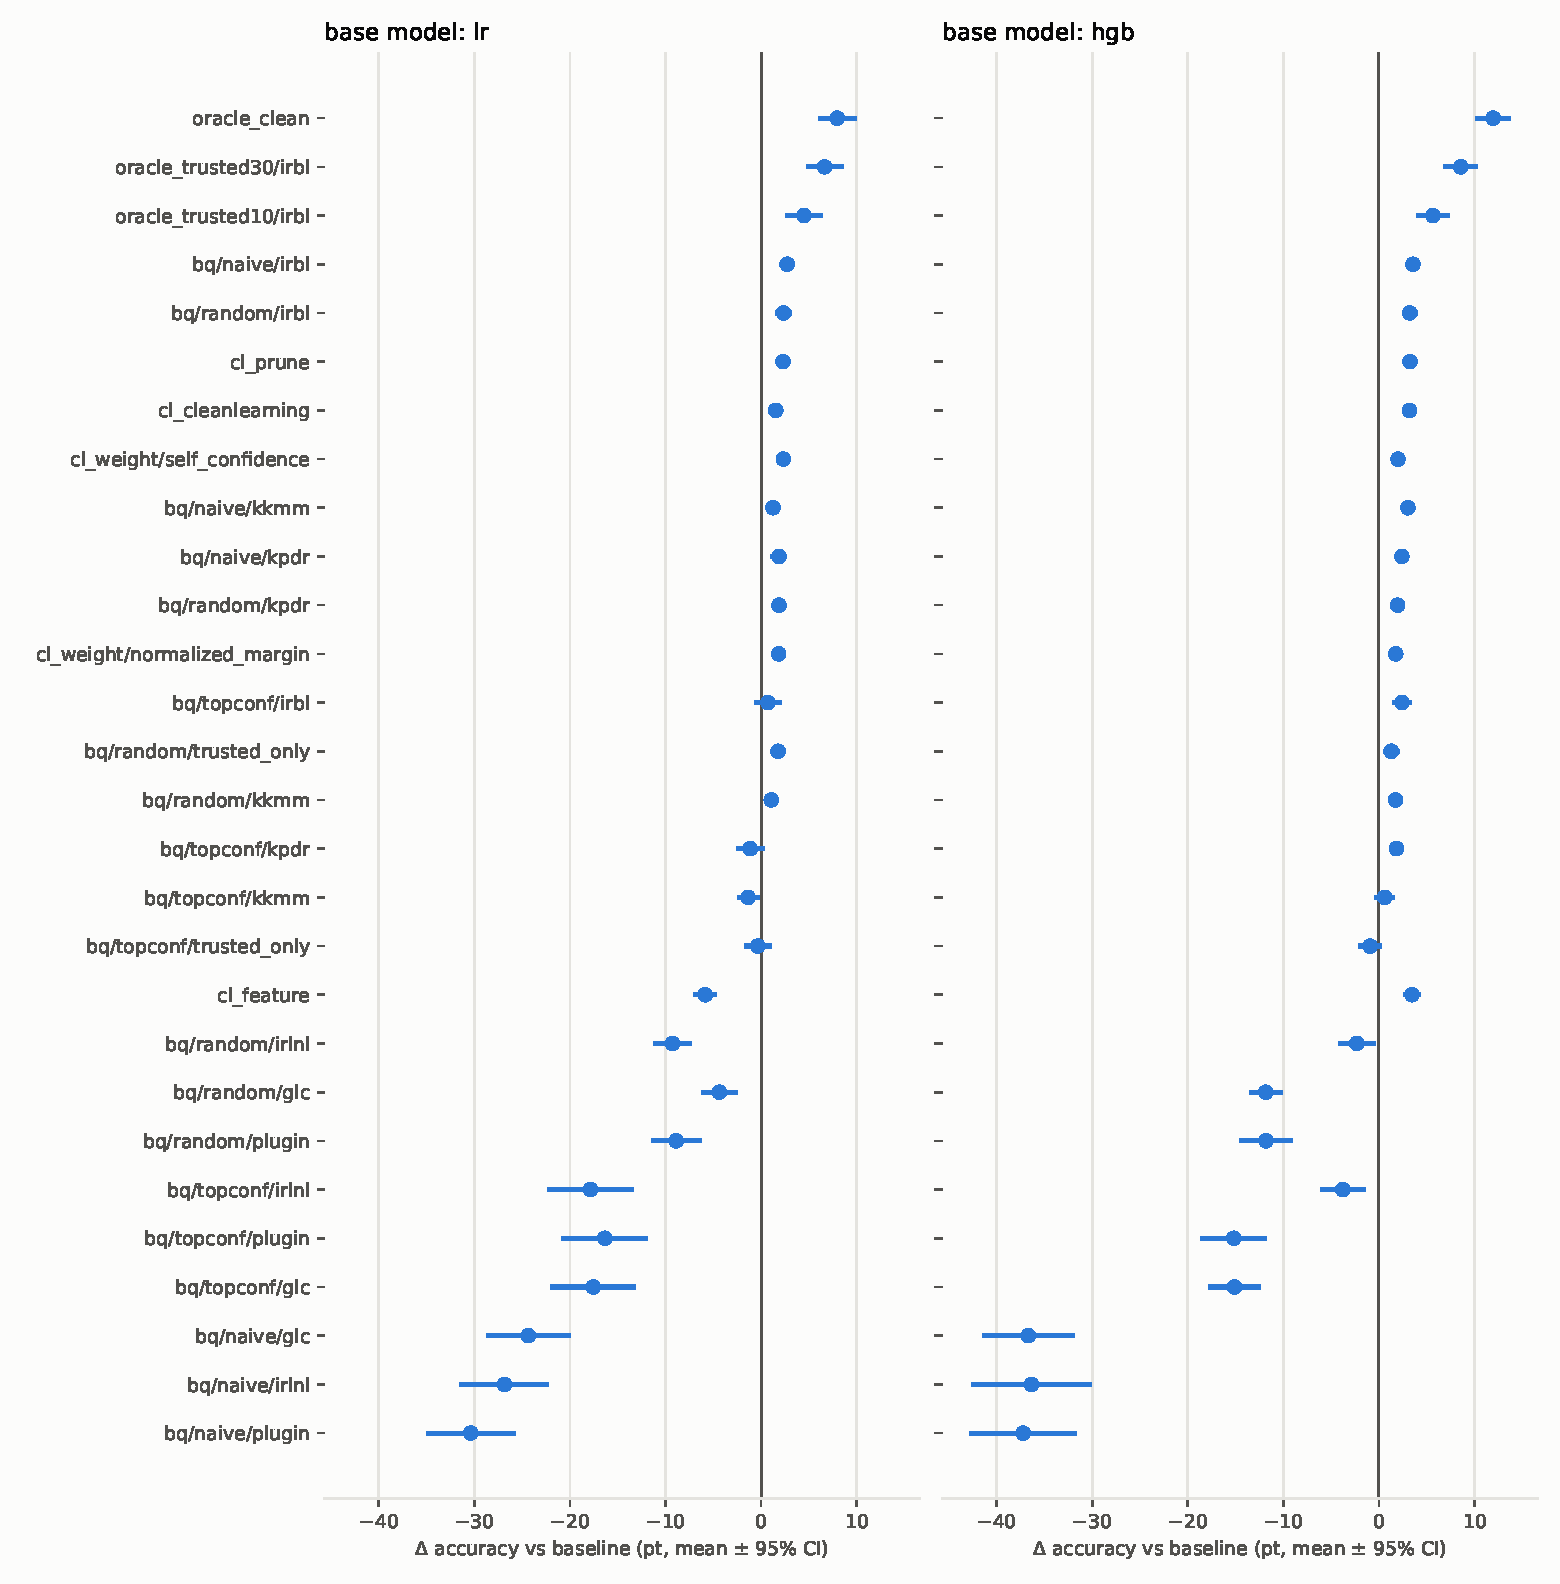
\includegraphics[width=\textwidth]{figures/delta_vs_baseline.pdf}
  \caption{Mean accuracy difference from \method{baseline} with 95\% confidence intervals (left: LR, right: HGB).}
  \label{fig:delta}
\end{figure}

\subsection{Paired comparisons}
Table~\ref{tab:paired} shows accuracy differences between methods under identical conditions.
\method{bq/naive/irbl} outperformed \method{cl\_prune} by \PLRNaiveIrblVsPrune{}~pt for LR and \PHGBNaiveIrblVsPrune{}~pt for HGB on average, with win rates of \PLRNaiveIrblVsPruneWin\% and \PHGBNaiveIrblVsPruneWin\%, respectively.
The differences are small, but the confidence intervals exclude 0 for both models.
The training time was \TimeLRRatio{} times that of \method{cl\_prune} for LR and \TimeHGBRatio{} times for HGB.

Relative to \method{cl\_prune}, \method{cl\_cleanlearning} scored \PLRCLVsPrune{}~pt for LR (win rate \PLRCLVsPruneWin\%) and \PHGBCLVsPrune{}~pt for HGB (win rate \PHGBCLVsPruneWin\%).
Per-class reweighting lowered accuracy for LR and had almost no effect for HGB.
As a result, the gap between \method{bq/naive/irbl} and \method{cl\_cleanlearning} (LR \PLRNaiveIrblVsCL{}, HGB \PHGBNaiveIrblVsCL{}~pt) is larger than that to \method{cl\_prune}.

Among the splitting schemes, \method{random} consistently outperformed \method{topconf} (with IRBL, LR \PLRRandomIrblVsTopIrbl{} and HGB \PHGBRandomIrblVsTopIrbl{}~pt; with \method{trusted\_only}, LR \PLRRandomTVsTopT{} and HGB \PHGBRandomTVsTopT{}~pt).
\method{naive} slightly outperformed \method{random} (with IRBL, LR \PLRNaiveIrblVsRandomIrbl{} and HGB \PHGBNaiveIrblVsRandomIrbl{}~pt).
Looking at the gain of IRBL over training on $\mathcal{T}$ alone within each split, the gain with \method{random} is LR \PLRRandomIrblVsRandomT{} and HGB \PHGBRandomIrblVsRandomT{}~pt, larger than the gain with \method{naive} (the difference from \method{cl\_prune}).
In other words, the advantage of \method{naive} is due less to IRBL's weighting than to the larger size of $\mathcal{T}$ (Section~\ref{sec:discussion}).

Using the quality score as weights, \method{cl\_weight/self\_confidence} was on par with \method{cl\_prune} for LR (\PLRWeightVsPrune) and worse for HGB (\PHGBWeightVsPrune).
Using it as a feature, \method{cl\_feature} was on par with \method{cl\_prune} for HGB (\PHGBFeatureVsPrune) but much worse for LR (\PLRFeatureVsPrune).

\begin{table}[tbp]
  \centering
  \caption{Accuracy differences (pt) between method A and method B under identical conditions. A win is the percentage of conditions in which A outperformed B. Differences are computed from unrounded accuracies, so they may differ by 0.01~pt from the differences of the rounded values in Table~\ref{tab:overall}.}
  \label{tab:paired}
  \footnotesize
  \setlength{\tabcolsep}{4pt}
  \begin{tabular}{llrrrr}
\toprule
 & & \multicolumn{2}{c}{LR} & \multicolumn{2}{c}{HGB} \\
\cmidrule(lr){3-4} \cmidrule(lr){5-6}
Method A & Method B & A$-$B (95\% CI) & A win & A$-$B (95\% CI) & A win \\
\midrule
\texttt{bq/naive/irbl} & \texttt{cl\_prune} & +0.45 {\scriptsize$\pm$0.36} & 64 & +0.31 {\scriptsize$\pm$0.24} & 71 \\
\texttt{bq/naive/irbl} & \texttt{cl\_cleanlearning} & +1.20 {\scriptsize$\pm$0.40} & 76 & +0.37 {\scriptsize$\pm$0.24} & 72 \\
\texttt{cl\_cleanlearning} & \texttt{cl\_prune} & $-$0.75 {\scriptsize$\pm$0.22} & 17 & $-$0.06 {\scriptsize$\pm$0.17} & 37 \\
\texttt{bq/random/irbl} & \texttt{bq/random/trusted\_only} & +0.58 {\scriptsize$\pm$0.27} & 80 & +1.91 {\scriptsize$\pm$0.33} & 88 \\
\texttt{bq/naive/irbl} & \texttt{bq/random/irbl} & +0.38 {\scriptsize$\pm$0.24} & 66 & +0.34 {\scriptsize$\pm$0.28} & 68 \\
\texttt{bq/random/irbl} & \texttt{bq/topconf/irbl} & +1.65 {\scriptsize$\pm$0.76} & 72 & +0.80 {\scriptsize$\pm$0.35} & 69 \\
\texttt{bq/random/trusted\_only} & \texttt{bq/topconf/trusted\_only} & +2.13 {\scriptsize$\pm$0.85} & 70 & +2.24 {\scriptsize$\pm$0.50} & 86 \\
\texttt{cl\_weight/self\_confidence} & \texttt{cl\_prune} & +0.04 {\scriptsize$\pm$0.28} & 57 & $-$1.26 {\scriptsize$\pm$0.47} & 30 \\
\texttt{cl\_feature} & \texttt{cl\_prune} & $-$8.14 {\scriptsize$\pm$1.14} & 2 & +0.21 {\scriptsize$\pm$0.50} & 47 \\
\texttt{oracle\_trusted10/irbl} & \texttt{bq/naive/irbl} & +1.75 {\scriptsize$\pm$1.32} & 41 & +2.08 {\scriptsize$\pm$1.29} & 44 \\
\texttt{oracle\_trusted30/irbl} & \texttt{bq/naive/irbl} & +3.91 {\scriptsize$\pm$1.35} & 72 & +5.00 {\scriptsize$\pm$1.38} & 92 \\
\texttt{oracle\_trusted30/irbl} & \texttt{oracle\_trusted10/irbl} & +2.16 {\scriptsize$\pm$0.32} & 99 & +2.92 {\scriptsize$\pm$0.58} & 96 \\
\bottomrule
\end{tabular}

\end{table}

\subsection{Differences by noise kind}
Table~\ref{tab:noise} shows $\Delta$ by noise kind and rate.
The automatic methods improved most under pair noise: at a noise rate of 40\%, \method{bq/naive/irbl} gained +6.91~pt for LR and +7.48~pt for HGB.
Under the same condition, however, \method{oracle\_trusted10/irbl} gained +19.94 (LR) and +21.40~pt (HGB), and \method{oracle\_trusted30/irbl} gained +21.95 (LR) and +24.22~pt (HGB), showing that using human-verified samples as the trusted set is extremely effective.
Under instance noise the automatic methods improved little; for LR, no method gained more than 1~pt.
For LR at instance 40\%, \method{bq/naive/irbl} ($-$0.18) fell below \method{cl\_prune} (+0.76) (see Section~\ref{sec:mech} for why).
The shortfall of \method{cl\_cleanlearning} relative to \method{cl\_prune} was largest for LR under symmetric noise (+0.68 vs.\ +2.21 at 40\%).

On average over all conditions \method{oracle\_trusted10/irbl} outperformed \method{bq/naive/irbl}, but its per-condition win rate was below half (LR \PLROracleTenVsNaiveIrblWin\%, HGB \PHGBOracleTenVsNaiveIrblWin\%), and most of the mean difference comes from pair noise at 40\%.
In contrast, with the trusted-set size matched at 30\%, \method{oracle\_trusted30/irbl} outperformed \method{bq/naive/irbl} by \PLROracleThirtyVsNaiveIrbl{}~pt for LR (win rate \PLROracleThirtyVsNaiveIrblWin\%) and \PHGBOracleThirtyVsNaiveIrbl{}~pt for HGB (win rate \PHGBOracleThirtyVsNaiveIrblWin\%).
Increasing the trusted set from 10\% to 30\% improved accuracy in almost every condition (win rate LR \PLROracleThirtyVsOracleTenWin\%, HGB \PHGBOracleThirtyVsOracleTenWin\%).

\begin{table}[tbp]
  \centering
  \caption{$\Delta$ by noise kind and rate (pt, mean over 3 datasets $\times$ 5 seeds). Main methods only. The first row is the accuracy of \method{baseline} (\%). All methods are listed in Table~\ref{tab:noise-all} in the appendix.}
  \label{tab:noise}
  \footnotesize
  \begin{tabular}{lrrrrrr}
\toprule
\multicolumn{7}{l}{\textbf{LR}} \\
 & \multicolumn{2}{c}{symmetric} & \multicolumn{2}{c}{pair} & \multicolumn{2}{c}{instance} \\
\cmidrule(lr){2-3} \cmidrule(lr){4-5} \cmidrule(lr){6-7}
 & 20\% & 40\% & 20\% & 40\% & 20\% & 40\% \\
\midrule
\textit{baseline acc.\ (\%)} & 77.91 & 75.63 & 73.27 & 58.20 & 78.35 & 75.51 \\
\addlinespace
\texttt{oracle\_clean} & +3.19 & +5.47 & +7.83 & +22.90 & +2.74 & +5.58 \\
\texttt{oracle\_trusted10/irbl} & +0.25 & +2.26 & +5.36 & +19.94 & $-$1.33 & +0.39 \\
\texttt{oracle\_trusted30/irbl} & +2.33 & +4.37 & +7.17 & +21.95 & +1.07 & +2.93 \\
\texttt{cl\_prune} & +1.61 & +2.21 & +4.54 & +3.87 & +0.70 & +0.76 \\
\texttt{cl\_cleanlearning} & +0.64 & +0.68 & +4.17 & +2.92 & +0.46 & +0.30 \\
\texttt{bq/naive/irbl} & +1.92 & +2.16 & +5.37 & +6.91 & +0.19 & $-$0.18 \\
\texttt{bq/random/irbl} & +1.83 & +2.15 & +5.25 & +5.33 & +0.04 & $-$0.50 \\
\texttt{bq/topconf/irbl} & $-$0.38 & +0.14 & +3.01 & +3.26 & $-$1.12 & $-$0.73 \\
\texttt{bq/naive/kpdr} & +0.86 & +0.74 & +4.39 & +5.77 & $-$0.48 & $-$0.18 \\
\texttt{cl\_weight/self\_confidence} & +2.31 & +2.98 & +3.78 & +3.17 & +1.00 & +0.67 \\
\texttt{cl\_feature} & $-$5.31 & $-$10.40 & $-$6.07 & $-$8.97 & $-$1.66 & $-$2.76 \\
\texttt{bq/random/glc} & $-$7.05 & $-$6.73 & $-$1.49 & $-$8.55 & $-$1.59 & $-$0.78 \\
\texttt{bq/naive/glc} & $-$38.60 & $-$32.27 & $-$32.78 & $-$25.11 & $-$9.75 & $-$7.66 \\
\midrule
\multicolumn{7}{l}{\textbf{HGB}} \\
 & \multicolumn{2}{c}{symmetric} & \multicolumn{2}{c}{pair} & \multicolumn{2}{c}{instance} \\
\cmidrule(lr){2-3} \cmidrule(lr){4-5} \cmidrule(lr){6-7}
 & 20\% & 40\% & 20\% & 40\% & 20\% & 40\% \\
\midrule
\textit{baseline acc.\ (\%)} & 85.61 & 78.68 & 82.35 & 61.36 & 81.64 & 71.91 \\
\addlinespace
\texttt{oracle\_clean} & +3.26 & +10.19 & +6.52 & +27.51 & +7.23 & +16.96 \\
\texttt{oracle\_trusted10/irbl} & $-$0.45 & +4.44 & +2.61 & +21.40 & +0.15 & +5.68 \\
\texttt{oracle\_trusted30/irbl} & +1.68 & +6.69 & +4.18 & +24.22 & +3.69 & +10.90 \\
\texttt{cl\_prune} & +0.51 & +5.23 & +2.99 & +7.13 & +0.46 & +3.19 \\
\texttt{cl\_cleanlearning} & +0.46 & +5.07 & +2.85 & +6.70 & +0.83 & +3.23 \\
\texttt{bq/naive/irbl} & +1.29 & +5.27 & +3.73 & +7.48 & +0.92 & +2.67 \\
\texttt{bq/random/irbl} & +0.76 & +4.85 & +3.19 & +7.36 & +0.23 & +2.93 \\
\texttt{bq/topconf/irbl} & $-$0.55 & +4.11 & +2.09 & +7.06 & $-$0.83 & +2.61 \\
\texttt{bq/naive/kpdr} & +0.72 & +3.14 & +2.89 & +6.06 & $-$0.18 & +1.74 \\
\texttt{cl\_weight/self\_confidence} & +0.88 & +3.61 & +2.16 & +3.09 & +0.78 & +1.43 \\
\texttt{cl\_feature} & $-$0.46 & +4.51 & +2.63 & +9.97 & +0.34 & +3.74 \\
\texttt{bq/random/glc} & $-$11.19 & $-$18.30 & $-$16.12 & $-$15.62 & $-$6.65 & $-$3.18 \\
\texttt{bq/naive/glc} & $-$53.12 & $-$40.74 & $-$52.48 & $-$26.30 & $-$26.29 & $-$21.20 \\
\bottomrule
\end{tabular}

\end{table}

\subsection{Detection performance of \cl{} and quality of the splits}\label{sec:diag}
Table~\ref{tab:diag} shows the detection performance of \cl{} and the error rates within each split.
Recall was high, 84--91\%, under symmetric noise and pair noise at 20\%, but only \InstRecallMin--\InstRecallMax\% under instance noise (range of means per dataset and model).
The error rate of the \method{naive} untrusted set (= the flagged samples) was \NaiveUntrustedMin--\NaiveUntrustedMax\%, and 2--26\% of the labels in the \method{naive} trusted set were still wrong, depending on the condition.
The untrusted sets of \method{random} and \method{topconf} also have error rates above $\rho$ because all of $\mathcal{I}$ goes into them (23--28\% at $\rho = 20\%$ and 45--54\% at $\rho = 40\%$).
The trusted set of \method{topconf} has a lower error rate than that of \method{random} (e.g., 1.2\% vs.\ 3.1\% for HGB with symmetric noise at 20\%).
Nevertheless, as shown above, \method{random} achieved higher accuracy.

\begin{table}[tbp]
  \centering
  \caption{Detection performance of \cl{} and error rates of the pseudo splits (\%, mean over 3 datasets $\times$ 5 seeds). Flagged is the fraction of samples flagged as errors. T is trusted and U is untrusted. For \method{naive}, $\mathcal{U} = \mathcal{I}$, so the error rate of naive U equals the precision, and the size of naive T is 1 $-$ the flagged fraction.}
  \label{tab:diag}
  \footnotesize
  \setlength{\tabcolsep}{3.5pt}
  \begin{tabular}{lllrrrrrrrrr}
\toprule
 & & & \multicolumn{3}{c}{cleanlab detection} & \multicolumn{2}{c}{naive} & \multicolumn{2}{c}{random} & \multicolumn{2}{c}{topconf} \\
\cmidrule(lr){4-6} \cmidrule(lr){7-8} \cmidrule(lr){9-10} \cmidrule(lr){11-12}
Model & Noise & Rate & Flagged & Prec. & Recall & T & U & T & U & T & U \\
\midrule
LR & symmetric & 20\% & 28.8 & 62.9 & 88.2 & 3.4 & 62.9 & 4.2 & 26.6 & 1.7 & 27.6 \\
 & symmetric & 40\% & 42.6 & 80.1 & 85.0 & 10.4 & 80.1 & 12.2 & 51.3 & 5.7 & 53.9 \\
 & pair & 20\% & 31.3 & 53.9 & 83.7 & 4.8 & 53.9 & 5.6 & 26.0 & 2.6 & 27.3 \\
 & pair & 40\% & 45.1 & 58.1 & 65.4 & 25.2 & 58.1 & 27.9 & 45.1 & 23.3 & 47.0 \\
 & instance & 20\% & 18.7 & 55.5 & 48.7 & 12.7 & 55.5 & 13.0 & 23.0 & 4.8 & 26.5 \\
 & instance & 40\% & 27.8 & 78.9 & 55.6 & 24.4 & 78.9 & 25.3 & 46.3 & 11.1 & 52.4 \\
\addlinespace
HGB & symmetric & 20\% & 26.0 & 71.8 & 91.4 & 2.4 & 71.8 & 3.1 & 27.1 & 1.2 & 27.9 \\
 & symmetric & 40\% & 44.4 & 79.9 & 88.6 & 8.2 & 79.9 & 10.2 & 52.4 & 5.6 & 54.3 \\
 & pair & 20\% & 27.6 & 63.2 & 86.4 & 3.8 & 63.2 & 5.2 & 26.3 & 2.5 & 27.4 \\
 & pair & 40\% & 45.7 & 56.3 & 64.3 & 26.2 & 56.3 & 28.2 & 45.1 & 23.4 & 47.1 \\
 & instance & 20\% & 20.7 & 61.4 & 61.0 & 9.9 & 61.4 & 9.9 & 24.3 & 3.4 & 27.1 \\
 & instance & 40\% & 30.7 & 73.0 & 56.2 & 25.2 & 73.0 & 26.5 & 45.8 & 14.7 & 50.8 \\
\bottomrule
\end{tabular}

\end{table}

\subsection{Control experiment: genuine trusted data}\label{sec:oracle}
To separate the degradation caused by pseudo trusted data from the performance of the methods themselves, we restored the true labels of 10\% or 30\% of the samples chosen uniformly at random, used them as the trusted set, and evaluated the same algorithms (Table~\ref{tab:oracle}).
The weighting methods IRBL and K-PDR performed best with oracle data and kept positive gains with naive and random.
\method{trusted\_only} reached only \OHGBTRUSTEDONLYTen{} for HGB with 10\% oracle data, but LR \OLRTRUSTEDONLYThirty{} and HGB \OHGBTRUSTEDONLYThirty{} with 30\%, so the size of the trusted set strongly affected the result.

The transition-matrix methods fell below \method{baseline} in most cases even with oracle data (GLC: LR \OLRGLCTen{} and HGB \OHGBGLCTen{} at 10\%, LR \OLRGLCThirty{} and HGB \OHGBGLCThirty{} at 30\%).
The exception was IRLNL with HGB, which improved by \OHGBIRLNLThirty{} at 30\%.
The degradation with \method{naive} ($-$24 to $-$37~pt), however, was far larger than with oracle data.
That is, the transition-matrix methods are not strong in our setting to begin with, and pseudo trusted data makes them much worse.

We initially hypothesized that the transition-matrix methods are weak even with oracle data because estimation is unstable for minority classes with few trusted samples (covtype).
The breakdown by dataset (Table~\ref{tab:oracle-breakdown}) shows that the degradation of Plugin is concentrated on covtype (around $-$20~pt for LR), consistent with this hypothesis.
GLC and IRLNL, however, also degrade for LR on the class-balanced synth (GLC down to $-$4.3~pt, IRLNL $-$18 to $-$24~pt under symmetric and instance noise), which minority classes alone cannot explain.
Since GLC's estimate of the diagonal barely changed when the trusted set grew from 10\% to 30\% (Section~\ref{sec:mech}), bias in the estimate rather than the number of samples appears to be the main factor.

\begin{table}[tbp]
  \centering
  \caption{$\Delta$ (pt) by how the trusted set is built. naive and random are pseudo trusted sets from \cl{}; oracle10 and oracle30 are genuine trusted sets in which 10\% or 30\% of the samples, chosen uniformly at random, have their true labels restored. $^\dagger$ \method{bq/naive/trusted\_only} is identical to \method{cl\_prune}, so its value is shown.}
  \label{tab:oracle}
  \footnotesize
  \begin{tabular}{lrrrrrrrr}
\toprule
 & \multicolumn{4}{c}{LR} & \multicolumn{4}{c}{HGB} \\
\cmidrule(lr){2-5} \cmidrule(lr){6-9}
Algorithm & naive & random & oracle10 & oracle30 & naive & random & oracle10 & oracle30 \\
\midrule
\texttt{trusted\_only} & +2.28$^\dagger$ & +1.77 & +3.45 & +6.47 & +3.25$^\dagger$ & +1.31 & $-$0.16 & +6.81 \\
\texttt{irbl} & +2.73 & +2.35 & +4.48 & +6.64 & +3.56 & +3.22 & +5.64 & +8.56 \\
\texttt{kpdr} & +1.85 & +1.86 & +3.11 & +6.14 & +2.40 & +1.95 & +4.49 & +7.17 \\
\texttt{glc} & $-$24.36 & $-$4.37 & $-$2.62 & $-$0.85 & $-$36.69 & $-$11.84 & $-$11.78 & $-$6.06 \\
\texttt{plugin} & $-$30.37 & $-$8.89 & $-$2.97 & $-$3.58 & $-$37.23 & $-$11.81 & $-$2.46 & $-$2.23 \\
\texttt{irlnl} & $-$26.86 & $-$9.27 & $-$10.82 & $-$8.93 & $-$36.34 & $-$2.32 & $-$1.31 & +5.08 \\
\bottomrule
\end{tabular}

\end{table}

\begin{table}[tbp]
  \centering
  \caption{$\Delta$ (pt) with genuine trusted data, broken down by dataset and noise (mean over 2 noise rates $\times$ 5 seeds). sym = symmetric, inst = instance.}
  \label{tab:oracle-breakdown}
  \scriptsize
  \setlength{\tabcolsep}{3.5pt}
  \begin{tabular}{llrrrrrrrrr}
\toprule
 & & \multicolumn{3}{c}{covtype} & \multicolumn{3}{c}{digits} & \multicolumn{3}{c}{synth} \\
\cmidrule(lr){3-5} \cmidrule(lr){6-8} \cmidrule(lr){9-11}
Algorithm & trusted & sym & pair & inst & sym & pair & inst & sym & pair & inst \\
\midrule
\multicolumn{11}{l}{\textbf{LR}} \\
\texttt{irbl} & 10\% & $-$0.4 & +3.3 & $-$2.1 & +4.7 & +23.2 & +2.9 & $-$0.6 & +11.4 & $-$2.2 \\
 & 30\% & +1.2 & +5.0 & $-$0.2 & +8.0 & +25.9 & +6.5 & +0.9 & +12.7 & $-$0.3 \\
\texttt{glc} & 10\% & $-$4.6 & $-$5.1 & $-$5.1 & +0.2 & +0.4 & +0.2 & $-$4.3 & $-$1.7 & $-$3.6 \\
 & 30\% & $-$10.1 & $-$2.7 & $-$3.5 & +2.3 & +10.2 & +2.4 & $-$3.4 & +0.0 & $-$2.8 \\
\texttt{plugin} & 10\% & $-$19.6 & $-$8.2 & $-$2.7 & $-$1.5 & +2.9 & $-$0.3 & $-$0.7 & +3.7 & $-$0.2 \\
 & 30\% & $-$20.2 & $-$8.7 & $-$2.3 & $-$4.4 & +3.6 & $-$2.1 & $-$1.0 & +3.2 & $-$0.2 \\
\texttt{irlnl} & 10\% & $-$4.5 & $-$11.5 & $-$7.9 & $-$13.2 & $-$0.8 & $-$3.0 & $-$21.2 & $-$11.6 & $-$23.7 \\
 & 30\% & $-$10.1 & $-$11.4 & $-$6.5 & $-$11.3 & +6.4 & $-$1.3 & $-$19.1 & $-$8.9 & $-$18.1 \\
\midrule\multicolumn{11}{l}{\textbf{HGB}} \\
\texttt{irbl} & 10\% & $-$1.9 & +6.1 & $-$0.8 & +4.2 & +16.2 & +3.9 & +3.6 & +13.7 & +5.6 \\
 & 30\% & +0.9 & +7.3 & +4.1 & +5.5 & +19.1 & +8.4 & +6.1 & +16.1 & +9.3 \\
\texttt{glc} & 10\% & $-$14.6 & $-$20.5 & $-$12.5 & $-$12.4 & $-$11.5 & $-$9.5 & $-$5.2 & $-$10.6 & $-$9.1 \\
 & 30\% & $-$9.2 & $-$8.0 & $-$8.2 & $-$6.7 & $-$2.1 & $-$4.2 & $-$3.0 & $-$7.0 & $-$6.1 \\
\texttt{plugin} & 10\% & $-$9.5 & $-$10.6 & $-$6.0 & $-$0.4 & +2.2 & $-$0.6 & $-$0.9 & +3.8 & $-$0.1 \\
 & 30\% & $-$8.6 & $-$4.4 & $-$1.5 & $-$2.9 & $-$0.7 & $-$1.6 & $-$2.3 & +2.2 & $-$0.3 \\
\texttt{irlnl} & 10\% & $-$1.7 & $-$16.5 & $-$13.1 & +2.2 & +4.8 & +1.9 & +2.5 & +5.6 & +2.5 \\
 & 30\% & +0.1 & +3.9 & +2.0 & +4.1 & +11.5 & +4.8 & +3.9 & +10.2 & +5.2 \\
\bottomrule
\end{tabular}

\end{table}

\subsection{Mechanism analysis}\label{sec:mech}
For all \NCond{} conditions and both models, we examined the transition matrices estimated by GLC (Table~\ref{tab:mech-glc}) and the weights IRBL assigned to the untrusted samples (Table~\ref{tab:mech-irbl}).

\paragraph{Estimating the transition matrix}
While the mean diagonal of the true transition matrix is \MechLRTrueDiag{}, the value estimated from \method{naive} was \MechLRNaiveDiag{} for LR and \MechHGBNaiveDiag{} for HGB.
Because the \texttt{gold} estimator uses a classifier trained on $\mathcal{U}$, the estimate reflects the noise in $\mathcal{U}$ rather than in the whole dataset.
The fraction of correct labels in the \method{naive} $\mathcal{U}$ is only \MechLRNaiveUClean{} for LR and \MechHGBNaiveUClean{} for HGB, and the estimate fell even below that.
Since $\mathcal{U} = \mathcal{I}$ consists solely of samples whose observed labels disagreed with the model's predictions, a classifier trained on $\mathcal{U}$ tends to learn a mapping opposite to the labels of $\mathcal{T}$.
This leads to a large overestimate of the noise, and the correction based on it appears to rewrite predictions in the wrong direction.
With \method{random}, unflagged samples mixed into $\mathcal{U}$ raise its clean rate to \MechLRRandomUClean{}, and the estimate improves to LR \MechLRRandomDiag{} and HGB \MechHGBRandomDiag{}.

Even with genuine trusted data, the estimate fell below the clean rate of $\mathcal{U}$ (\MechLROracleTenUClean{}): \MechLROracleTenDiag{} for LR and \MechHGBOracleTenDiag{} for HGB.
Increasing the trusted set to 30\% left the estimate almost unchanged (LR \MechLROracleThirtyDiag{}, HGB \MechHGBOracleThirtyDiag{}).
The \texttt{gold} estimator assumes that the classifier trained on $\mathcal{U}$ accurately represents the posterior of the noisy labels.
If the classifier's predicted probabilities are not concentrated on the true class, the diagonal is estimated below 1 even without noise, so the classifier's own error appears to be added on top of the noise.
That the underestimate is larger for LR and smaller for the more expressive HGB is consistent with this interpretation.
For HGB, however, the accuracy drop of GLC is larger than for LR even though its estimate is close to the true value (Table~\ref{tab:oracle}), which the bias of the estimate alone cannot explain.
Other factors, such as an interaction with training after the correction, are likely involved, but we have not identified them.

\paragraph{IRBL weights}
IRBL assigned to the \method{naive} untrusted samples whose labels are actually wrong a mean weight of \MechLRWNoisy{} (LR) and \MechHGBWNoisy{} (HGB), and to those whose labels are actually correct \MechLRWClean{} (LR) and \MechHGBWClean{} (HGB).
That is, rather than discarding all flagged samples, IRBL recovered \cl{}'s false positives (samples flagged as errors even though their labels are correct).
This appears to be the reason for its slight advantage over \method{cl\_prune}.
The absolute weights differ between models, but the ratio of the weights on correct and wrong labels decreased in the order \method{naive} (LR 6.1, HGB 5.6), \method{random} (3.4, 4.9), and \method{topconf} (2.6, 4.1).
With \method{topconf}, the trusted set is biased toward easy samples, which apparently makes it harder for IRBL to tell wrong labels from ``hard but correct'' ones, consistent with the results for RQ2.

For LR at instance 40\%, the mean weight on the wrong labels in the \method{naive} untrusted set was 0.80, barely lower than for correct labels and in contrast to symmetric noise (0.04--0.09).
Instance noise consists of errors that look natural to LR, and 24\% of the labels in the \method{naive} trusted set remain wrong, so IRBL cannot tell the errors apart.
This appears to be why \method{bq/naive/irbl} fell below \method{cl\_prune} in this condition.

\begin{table}[tbp]
  \centering
  \caption{Mean diagonal of the transition matrix estimated by GLC (\texttt{gold}) and the fraction of correct labels in the untrusted set (mean over 3 datasets $\times$ 5 seeds). True is the unweighted average over classes of the diagonal of the true transition matrix of the whole dataset, $\frac{1}{K}\sum_{k} T_{kk}$. Under instance noise, flips concentrate on error-prone classes, so it does not match the sample-level noise rate $\rho$.}
  \label{tab:mech-glc}
  \scriptsize
  \setlength{\tabcolsep}{3.5pt}
  \begin{tabular}{lllrrrrrrrrr}
\toprule
 & & & \multicolumn{5}{c}{Mean diagonal estimated by GLC} & \multicolumn{3}{c}{Clean rate of U} \\
\cmidrule(lr){4-8} \cmidrule(lr){9-11}
Model & Noise & Rate & True & naive & random & topconf & oracle10 & oracle30 & naive & random & oracle10 \\
\midrule
LR & symmetric & 20\% & 0.80 & 0.12 & 0.42 & 0.47 & 0.49 & 0.49 & 0.37 & 0.73 & 0.80 \\
 & symmetric & 40\% & 0.60 & 0.10 & 0.27 & 0.24 & 0.37 & 0.37 & 0.20 & 0.49 & 0.60 \\
 & pair & 20\% & 0.80 & 0.19 & 0.47 & 0.53 & 0.50 & 0.49 & 0.46 & 0.74 & 0.80 \\
 & pair & 40\% & 0.60 & 0.25 & 0.37 & 0.39 & 0.38 & 0.38 & 0.42 & 0.55 & 0.60 \\
 & instance & 20\% & 0.78 & 0.34 & 0.68 & 0.80 & 0.65 & 0.64 & 0.45 & 0.77 & 0.80 \\
 & instance & 40\% & 0.57 & 0.36 & 0.64 & 0.75 & 0.60 & 0.60 & 0.21 & 0.54 & 0.60 \\
\addlinespace
HGB & symmetric & 20\% & 0.80 & 0.11 & 0.61 & 0.66 & 0.68 & 0.68 & 0.28 & 0.73 & 0.80 \\
 & symmetric & 40\% & 0.60 & 0.11 & 0.39 & 0.38 & 0.53 & 0.53 & 0.20 & 0.48 & 0.60 \\
 & pair & 20\% & 0.80 & 0.14 & 0.62 & 0.68 & 0.67 & 0.66 & 0.37 & 0.74 & 0.80 \\
 & pair & 40\% & 0.60 & 0.28 & 0.45 & 0.44 & 0.49 & 0.49 & 0.44 & 0.55 & 0.60 \\
 & instance & 20\% & 0.78 & 0.31 & 0.76 & 0.84 & 0.72 & 0.71 & 0.39 & 0.76 & 0.80 \\
 & instance & 40\% & 0.57 & 0.31 & 0.69 & 0.77 & 0.63 & 0.63 & 0.27 & 0.54 & 0.60 \\
\bottomrule
\end{tabular}

\end{table}

\begin{table}[tbp]
  \centering
  \caption{Mean weights assigned by IRBL to untrusted samples (mean over 3 datasets $\times$ 5 seeds). Noisy and Clean denote untrusted samples whose labels are actually wrong and correct, respectively.}
  \label{tab:mech-irbl}
  \footnotesize
  \begin{tabular}{lllrrrrrr}
\toprule
 & & & \multicolumn{2}{c}{naive} & \multicolumn{2}{c}{random} & \multicolumn{2}{c}{topconf} \\
\cmidrule(lr){4-5} \cmidrule(lr){6-7} \cmidrule(lr){8-9}
Model & Noise & Rate & Noisy & Clean & Noisy & Clean & Noisy & Clean \\
\midrule
LR & symmetric & 20\% & 0.04 & 1.48 & 0.14 & 1.42 & 0.33 & 1.35 \\
 & symmetric & 40\% & 0.09 & 2.32 & 0.19 & 2.04 & 0.29 & 1.96 \\
 & pair & 20\% & 0.06 & 2.07 & 0.18 & 1.38 & 0.31 & 1.36 \\
 & pair & 40\% & 0.25 & 1.81 & 0.49 & 1.33 & 0.52 & 1.26 \\
 & instance & 20\% & 0.65 & 1.29 & 0.72 & 1.04 & 0.85 & 1.05 \\
 & instance & 40\% & 0.80 & 2.53 & 0.74 & 1.17 & 0.83 & 1.21 \\
\addlinespace
HGB & symmetric & 20\% & 0.01 & 0.36 & 0.03 & 0.91 & 0.05 & 0.82 \\
 & symmetric & 40\% & 0.02 & 0.53 & 0.05 & 0.98 & 0.06 & 0.92 \\
 & pair & 20\% & 0.02 & 0.46 & 0.07 & 0.89 & 0.09 & 0.81 \\
 & pair & 40\% & 0.17 & 0.54 & 0.28 & 0.75 & 0.28 & 0.70 \\
 & instance & 20\% & 0.12 & 0.37 & 0.31 & 0.87 & 0.36 & 0.80 \\
 & instance & 40\% & 0.15 & 0.48 & 0.35 & 0.90 & 0.35 & 0.86 \\
\bottomrule
\end{tabular}

\end{table}

\section{Discussion}\label{sec:discussion}

\paragraph{RQ1: Is pseudo-biquality learning better than pruning?}
Only in combination with weighting methods, IRBL in particular, did it slightly outperform pruning.
The improvement is small, 0.3--0.5~pt, and the training time is about three times longer.
\cl{}'s standard \texttt{CleanLearning} removes the same samples and only adds per-class reweighting, yet it did not outperform \method{cl\_prune}.
Since the shortfall was largest for LR under symmetric noise, where the noise rate does not depend on the class, variation in the estimated per-class noise rates may have introduced spurious bias between classes.
The advantage of \method{bq/naive/irbl} therefore cannot be explained by reweighting per se; it appears to lie in recovering falsely flagged samples individually.

The size of the trusted set, however, also contributes to the advantage of \method{naive}.
$\mathcal{T}$ of \method{naive} covers the majority of the training data, whereas that of \method{random} covers about 30\%.
Since the gain of IRBL over training on $\mathcal{T}$ alone was larger with \method{random}, IRBL's weighting itself works even with a small $\mathcal{T}$, and the benefit of \method{naive} appears to lie mainly in the size of $\mathcal{T}$.
Combinations with transition-matrix methods should be avoided.

\paragraph{RQ2: How to choose the trusted set}
\method{topconf}, which uses the samples with the top quality scores as trusted, lowered accuracy even though it lowered the error rate of the trusted set.
When the trusted set is biased toward ``samples that are easy for the model'', weighting methods end up weighting by ``easy or hard'', which apparently lowers the weights of hard but correct samples.
The measured IRBL weights (Table~\ref{tab:mech-irbl}) support this.
This is also consistent with the finding of Dataset Cartography~\cite{swayamdipta2020cartography} that confidence-based selection is biased toward easy-to-learn samples and that ambiguous samples contribute to generalization.
When building a pseudo trusted set, following the same distribution as the untrusted set should take priority over the cleanliness of the labels.

This tendency, however, depended on the dataset (Table~\ref{tab:dataset-all} in the appendix).
For LR on covtype, which is strongly imbalanced, every split that narrows the trusted set to 30\% of the training data fell below \method{baseline} (\method{bq/random/irbl} $-$0.53 and \method{bq/random/trusted\_only} $-$1.14~pt), and positive gains were limited to \method{bq/naive/irbl} (+0.53) and \method{cl\_prune} (+0.14).
For LR on digits, by contrast, \method{bq/topconf/irbl} (+7.01) outperformed \method{bq/random/irbl} (+5.41).
The disadvantage of narrowing the trusted set and the effect of selection bias appear to interact with the structure and class balance of the data.

\paragraph{RQ3: Using quality scores as weights or features}
Using the scores as weights was on par with or worse than pruning and showed no benefit.
Using them as a feature worked as well as pruning for HGB but degraded LR substantially.
We see three possible factors.
First, when $s$ is concatenated additively to a multiclass logistic regression, the logit of class $c$ becomes $w_c^\top x + w_{c,s} s + b_c$, so $s$ can only shift the logits independently of $x$.
It therefore cannot represent ``the decision boundary when the label is reliable''.
This is a limitation specific to additive concatenation without interaction terms (such as $s x$); a linear model can represent it if the interactions are added explicitly.
Second, $s$ is spread widely below 1 during training, whereas $s=1$ is given uniformly at inference.
If classes with a high average $s$ during training receive a positive $w_{c,s}$, a constant corresponding to $w_{c,s}(1 - \bar{s})$ is added to each class's intercept at inference, which may bias predictions toward those classes.
That LR degraded strongly even under symmetric noise ($-$5.31~pt at 20\% and $-$10.40~pt at 40\%) is consistent with this intercept shift.
Third, for HGB, splits on $s$ ($s > \theta$) route inputs at inference, where $s=1$, into subtrees built from high-confidence training samples.
This appears to act as implicit pruning inside the trees rather than learning a decision boundary conditioned on confidence.
We have not verified these explanations directly.

\paragraph{Practical implications}
If no human input is used at all, pruning with \cl{} is the first choice in terms of the balance between ease and effect.
In our experiments, the per-class reweighting of \texttt{CleanLearning} brought no additional gain.
If computation time allows, combining the \method{naive} split with IRBL can be expected to add a small gain.
On the other hand, if 30\% of the training data can be verified by hand, IRBL outperforms the best automatic method by about 4--5~pt on average, with a high win rate (LR \PLROracleThirtyVsNaiveIrblWin\%, HGB \PHGBOracleThirtyVsNaiveIrblWin\%).
With 10\% verification, it wins on average but in fewer than half of the conditions, although under heavy systematic noise (pair 40\%) it outperformed the automatic methods by 13--14~pt.
When the nature of the noise is unknown, it is worth verifying a small random sample to learn the noise rate and its tendencies.

\section{Limitations}\label{sec:limit}
\begin{itemize}
  \item All noise is synthetic. In particular, the instance noise was generated with LR, so it is biased toward directions that are hard for LR to detect, and the conditions are not symmetric between LR and HGB.
  \item We use only three small-to-medium tabular datasets and do not cover images, text, or deep learning models. The effect of narrowing the trusted set differs between datasets (covtype vs.\ digits), which limits generalization from three datasets.
  \item Hyperparameters ($\tau$, the detection settings of \cl{}, and the settings of each algorithm) were not tuned, and only a single value, $\tau = 0.3$, was evaluated.
  \item The HGB learning rate was originally chosen by referring to the test data. We confirmed post hoc that cross-validation within the training data leads to the same choice, but the selection process itself depended on the test data.
  \item We confirmed that the underestimate of the \texttt{gold} estimator and minority classes contribute to the weakness of the transition-matrix methods with genuine trusted data, but we have not identified what causes the degradation for HGB.
  \item The training time of \texttt{CleanLearning} includes re-running the label-issue detection internally, so it is not comparable with the other methods and is not reported.
  \item The confidence intervals do not account for correlations between conditions.
\end{itemize}

\section{Conclusion}
We evaluated pseudo-biquality learning, which builds trusted/untrusted sets automatically from \cl{}'s output and feeds them to \bq{}, on \NCond{} conditions $\times$ 2 models.
The combination with IRBL slightly outperformed pruning and \texttt{CleanLearning}, but part of this benefit came from the size of the trusted set.
Combinations with transition-matrix methods broke down badly, and we confirmed by measurement that the cause is the underestimated transition matrix resulting from mislabeled samples concentrating in the untrusted set.
For choosing the trusted set, low distributional bias mattered more than clean labels.
On the other hand, the gap to a human-verified trusted set of the same size was large, so the cost of removing humans entirely is not small.
Future work includes validation on real-world noise, a systematic exploration of the trusted-set ratio and selection, and semi-automatic schemes that combine a small amount of human verification with \cl{}.

\printbibliography

\appendix
\clearpage
\section{Detailed Results}

\begin{table}[htbp]
  \centering
  \caption{$\Delta$ by noise kind and rate (pt, all methods). The first row is the accuracy of \method{baseline} (\%).}
  \label{tab:noise-all}
  \scriptsize
  \setlength{\tabcolsep}{4pt}
  \begin{tabular}{lrrrrrr}
\toprule
\multicolumn{7}{l}{\textbf{LR}} \\
 & \multicolumn{2}{c}{symmetric} & \multicolumn{2}{c}{pair} & \multicolumn{2}{c}{instance} \\
\cmidrule(lr){2-3} \cmidrule(lr){4-5} \cmidrule(lr){6-7}
 & 20\% & 40\% & 20\% & 40\% & 20\% & 40\% \\
\midrule
\textit{baseline acc.\ (\%)} & 77.91 & 75.63 & 73.27 & 58.20 & 78.35 & 75.51 \\
\addlinespace
\texttt{oracle\_clean} & +3.19 & +5.47 & +7.83 & +22.90 & +2.74 & +5.58 \\
\texttt{oracle\_trusted10/irbl} & +0.25 & +2.26 & +5.36 & +19.94 & $-$1.33 & +0.39 \\
\texttt{oracle\_trusted30/irbl} & +2.33 & +4.37 & +7.17 & +21.95 & +1.07 & +2.93 \\
\texttt{cl\_prune} & +1.61 & +2.21 & +4.54 & +3.87 & +0.70 & +0.76 \\
\texttt{cl\_cleanlearning} & +0.64 & +0.68 & +4.17 & +2.92 & +0.46 & +0.30 \\
\texttt{bq/naive/irbl} & +1.92 & +2.16 & +5.37 & +6.91 & +0.19 & $-$0.18 \\
\texttt{bq/naive/kpdr} & +0.86 & +0.74 & +4.39 & +5.77 & $-$0.48 & $-$0.18 \\
\texttt{bq/naive/kkmm} & $-$0.23 & $-$1.04 & +3.80 & +5.80 & $-$0.39 & $-$0.49 \\
\texttt{bq/naive/glc} & $-$38.60 & $-$32.27 & $-$32.78 & $-$25.11 & $-$9.75 & $-$7.66 \\
\texttt{bq/naive/plugin} & $-$49.56 & $-$50.07 & $-$18.73 & $-$9.32 & $-$30.34 & $-$24.21 \\
\texttt{bq/naive/irlnl} & $-$46.12 & $-$37.07 & $-$34.85 & $-$23.44 & $-$10.67 & $-$8.99 \\
\texttt{bq/random/trusted\_only} & +1.16 & +1.73 & +4.16 & +3.11 & +0.07 & +0.41 \\
\texttt{bq/random/irbl} & +1.83 & +2.15 & +5.25 & +5.33 & +0.04 & $-$0.50 \\
\texttt{bq/random/kpdr} & +1.11 & +1.46 & +4.58 & +4.37 & $-$0.31 & $-$0.04 \\
\texttt{bq/random/kkmm} & +0.26 & +0.09 & +3.97 & +2.93 & $-$0.33 & $-$0.59 \\
\texttt{bq/random/glc} & $-$7.05 & $-$6.73 & $-$1.49 & $-$8.55 & $-$1.59 & $-$0.78 \\
\texttt{bq/random/plugin} & $-$14.21 & $-$19.88 & $-$6.63 & $-$9.83 & $-$1.22 & $-$1.61 \\
\texttt{bq/random/irlnl} & $-$15.52 & $-$9.67 & $-$6.85 & $-$9.39 & $-$8.91 & $-$5.27 \\
\texttt{bq/topconf/trusted\_only} & $-$2.17 & $-$1.46 & +1.34 & +0.81 & $-$1.12 & +0.48 \\
\texttt{bq/topconf/irbl} & $-$0.38 & +0.14 & +3.01 & +3.26 & $-$1.12 & $-$0.73 \\
\texttt{bq/topconf/kpdr} & $-$2.61 & $-$2.57 & $-$0.15 & +1.07 & $-$1.91 & $-$0.71 \\
\texttt{bq/topconf/kkmm} & $-$2.77 & $-$2.87 & $-$0.13 & +1.20 & $-$2.38 & $-$1.26 \\
\texttt{bq/topconf/glc} & $-$25.10 & $-$31.27 & $-$18.10 & $-$23.74 & $-$1.03 & $-$6.14 \\
\texttt{bq/topconf/plugin} & $-$20.05 & $-$33.94 & $-$15.53 & $-$21.52 & $-$2.15 & $-$4.93 \\
\texttt{bq/topconf/irlnl} & $-$28.06 & $-$31.56 & $-$14.00 & $-$23.08 & $-$4.49 & $-$6.01 \\
\texttt{cl\_weight/self\_confidence} & +2.31 & +2.98 & +3.78 & +3.17 & +1.00 & +0.67 \\
\texttt{cl\_weight/normalized\_margin} & +1.55 & +1.58 & +3.63 & +2.80 & +0.85 & +0.59 \\
\texttt{cl\_feature} & $-$5.31 & $-$10.40 & $-$6.07 & $-$8.97 & $-$1.66 & $-$2.76 \\
\midrule
\multicolumn{7}{l}{\textbf{HGB}} \\
 & \multicolumn{2}{c}{symmetric} & \multicolumn{2}{c}{pair} & \multicolumn{2}{c}{instance} \\
\cmidrule(lr){2-3} \cmidrule(lr){4-5} \cmidrule(lr){6-7}
 & 20\% & 40\% & 20\% & 40\% & 20\% & 40\% \\
\midrule
\textit{baseline acc.\ (\%)} & 85.61 & 78.68 & 82.35 & 61.36 & 81.64 & 71.91 \\
\addlinespace
\texttt{oracle\_clean} & +3.26 & +10.19 & +6.52 & +27.51 & +7.23 & +16.96 \\
\texttt{oracle\_trusted10/irbl} & $-$0.45 & +4.44 & +2.61 & +21.40 & +0.15 & +5.68 \\
\texttt{oracle\_trusted30/irbl} & +1.68 & +6.69 & +4.18 & +24.22 & +3.69 & +10.90 \\
\texttt{cl\_prune} & +0.51 & +5.23 & +2.99 & +7.13 & +0.46 & +3.19 \\
\texttt{cl\_cleanlearning} & +0.46 & +5.07 & +2.85 & +6.70 & +0.83 & +3.23 \\
\texttt{bq/naive/irbl} & +1.29 & +5.27 & +3.73 & +7.48 & +0.92 & +2.67 \\
\texttt{bq/naive/kpdr} & +0.72 & +3.14 & +2.89 & +6.06 & $-$0.18 & +1.74 \\
\texttt{bq/naive/kkmm} & +0.64 & +4.39 & +2.92 & +7.13 & +0.42 & +2.69 \\
\texttt{bq/naive/glc} & $-$53.12 & $-$40.74 & $-$52.48 & $-$26.30 & $-$26.29 & $-$21.20 \\
\texttt{bq/naive/plugin} & $-$62.42 & $-$57.03 & $-$21.08 & $-$5.88 & $-$43.67 & $-$33.31 \\
\texttt{bq/naive/irlnl} & $-$64.59 & $-$64.25 & $-$61.43 & $-$7.68 & $-$9.91 & $-$10.18 \\
\texttt{bq/random/trusted\_only} & $-$1.96 & +3.05 & $-$0.12 & +5.10 & $-$0.81 & +2.58 \\
\texttt{bq/random/irbl} & +0.76 & +4.85 & +3.19 & +7.36 & +0.23 & +2.93 \\
\texttt{bq/random/kpdr} & +0.44 & +2.85 & +2.06 & +4.92 & $-$0.03 & +1.47 \\
\texttt{bq/random/kkmm} & $-$0.38 & +2.81 & +1.79 & +4.80 & $-$0.29 & +1.72 \\
\texttt{bq/random/glc} & $-$11.19 & $-$18.30 & $-$16.12 & $-$15.62 & $-$6.65 & $-$3.18 \\
\texttt{bq/random/plugin} & $-$8.28 & $-$30.88 & $-$10.22 & $-$15.05 & $-$2.69 & $-$3.74 \\
\texttt{bq/random/irlnl} & $-$0.47 & $-$8.75 & $-$2.09 & $-$4.06 & +0.47 & +1.00 \\
\texttt{bq/topconf/trusted\_only} & $-$6.02 & +0.50 & $-$3.09 & +4.79 & $-$4.15 & +2.40 \\
\texttt{bq/topconf/irbl} & $-$0.55 & +4.11 & +2.09 & +7.06 & $-$0.83 & +2.61 \\
\texttt{bq/topconf/kpdr} & $-$0.26 & +2.74 & +1.49 & +5.90 & $-$0.99 & +2.12 \\
\texttt{bq/topconf/kkmm} & $-$3.31 & +1.95 & $-$0.51 & +5.64 & $-$2.65 & +2.50 \\
\texttt{bq/topconf/glc} & $-$13.33 & $-$24.31 & $-$19.80 & $-$21.87 & $-$5.44 & $-$5.95 \\
\texttt{bq/topconf/plugin} & $-$9.63 & $-$33.35 & $-$17.82 & $-$24.21 & $-$1.29 & $-$4.80 \\
\texttt{bq/topconf/irlnl} & $-$0.63 & $-$9.35 & $-$4.21 & $-$10.14 & +0.60 & +1.03 \\
\texttt{cl\_weight/self\_confidence} & +0.88 & +3.61 & +2.16 & +3.09 & +0.78 & +1.43 \\
\texttt{cl\_weight/normalized\_margin} & +0.48 & +2.49 & +2.09 & +3.21 & +0.65 & +1.63 \\
\texttt{cl\_feature} & $-$0.46 & +4.51 & +2.63 & +9.97 & +0.34 & +3.74 \\
\bottomrule
\end{tabular}

\end{table}

\begin{table}[htbp]
  \centering
  \caption{$\Delta$ by dataset (pt, all methods, mean over 3 noise kinds $\times$ 2 rates $\times$ 5 seeds). The first row is the accuracy of \method{baseline} (\%).}
  \label{tab:dataset-all}
  \scriptsize
  \begin{tabular}{lrrr}
\toprule
\multicolumn{4}{l}{\textbf{LR}} \\
 & covtype & digits & synth \\
\midrule
\textit{baseline acc.\ (\%)} & 69.71 & 80.95 & 68.77 \\
\addlinespace
\texttt{oracle\_clean} & +2.84 & +15.86 & +5.15 \\
\texttt{oracle\_trusted10/irbl} & +0.29 & +10.30 & +2.85 \\
\texttt{oracle\_trusted30/irbl} & +2.02 & +13.47 & +4.42 \\
\texttt{cl\_prune} & +0.14 & +5.48 & +1.22 \\
\texttt{cl\_cleanlearning} & $-$1.42 & +4.78 & +1.22 \\
\texttt{bq/naive/irbl} & +0.53 & +5.22 & +2.43 \\
\texttt{bq/naive/kpdr} & $-$0.43 & +5.54 & +0.45 \\
\texttt{bq/naive/kkmm} & $-$1.22 & +3.57 & +1.38 \\
\texttt{bq/naive/glc} & $-$10.10 & $-$36.83 & $-$26.15 \\
\texttt{bq/naive/plugin} & $-$29.51 & $-$40.50 & $-$21.11 \\
\texttt{bq/naive/irlnl} & $-$15.51 & $-$38.06 & $-$27.00 \\
\texttt{bq/random/trusted\_only} & $-$1.14 & +5.37 & +1.09 \\
\texttt{bq/random/irbl} & $-$0.53 & +5.41 & +2.17 \\
\texttt{bq/random/kpdr} & $-$0.69 & +4.48 & +1.79 \\
\texttt{bq/random/kkmm} & $-$1.14 & +2.85 & +1.46 \\
\texttt{bq/random/glc} & $-$9.26 & +0.90 & $-$4.73 \\
\texttt{bq/random/plugin} & $-$19.15 & $-$4.54 & $-$2.99 \\
\texttt{bq/random/irlnl} & $-$12.09 & $-$4.92 & $-$10.79 \\
\texttt{bq/topconf/trusted\_only} & $-$7.49 & +6.73 & $-$0.31 \\
\texttt{bq/topconf/irbl} & $-$5.89 & +7.01 & +0.98 \\
\texttt{bq/topconf/kpdr} & $-$7.53 & +5.72 & $-$1.63 \\
\texttt{bq/topconf/kkmm} & $-$6.64 & +3.33 & $-$0.79 \\
\texttt{bq/topconf/glc} & $-$37.62 & $-$2.01 & $-$13.07 \\
\texttt{bq/topconf/plugin} & $-$37.62 & $-$2.03 & $-$9.42 \\
\texttt{bq/topconf/irlnl} & $-$38.02 & $-$1.59 & $-$13.99 \\
\texttt{cl\_weight/self\_confidence} & +0.41 & +5.35 & +1.20 \\
\texttt{cl\_weight/normalized\_margin} & +0.18 & +4.32 & +1.00 \\
\texttt{cl\_feature} & $-$11.10 & $-$0.68 & $-$5.81 \\
\midrule
\multicolumn{4}{l}{\textbf{HGB}} \\
 & covtype & digits & synth \\
\midrule
\textit{baseline acc.\ (\%)} & 70.91 & 83.47 & 76.40 \\
\addlinespace
\texttt{oracle\_clean} & +8.87 & +13.64 & +13.33 \\
\texttt{oracle\_trusted10/irbl} & +1.15 & +8.11 & +7.65 \\
\texttt{oracle\_trusted30/irbl} & +4.14 & +11.03 & +10.51 \\
\texttt{cl\_prune} & +0.64 & +4.98 & +4.13 \\
\texttt{cl\_cleanlearning} & +0.51 & +5.04 & +4.02 \\
\texttt{bq/naive/irbl} & +1.36 & +4.91 & +4.41 \\
\texttt{bq/naive/kpdr} & +1.57 & +3.04 & +2.57 \\
\texttt{bq/naive/kkmm} & +1.04 & +4.51 & +3.54 \\
\texttt{bq/naive/glc} & $-$21.12 & $-$53.56 & $-$35.39 \\
\texttt{bq/naive/plugin} & $-$31.28 & $-$46.13 & $-$34.28 \\
\texttt{bq/naive/irlnl} & $-$31.70 & $-$41.78 & $-$35.54 \\
\texttt{bq/random/trusted\_only} & $-$1.44 & +3.09 & +2.27 \\
\texttt{bq/random/irbl} & +0.23 & +5.14 & +4.29 \\
\texttt{bq/random/kpdr} & +0.93 & +2.43 & +2.49 \\
\texttt{bq/random/kkmm} & $-$0.77 & +3.16 & +2.84 \\
\texttt{bq/random/glc} & $-$16.01 & $-$11.02 & $-$8.50 \\
\texttt{bq/random/plugin} & $-$20.98 & $-$8.23 & $-$6.22 \\
\texttt{bq/random/irlnl} & $-$8.68 & +0.83 & +0.90 \\
\texttt{bq/topconf/trusted\_only} & $-$3.79 & +0.81 & +0.18 \\
\texttt{bq/topconf/irbl} & $-$1.46 & +5.01 & +3.70 \\
\texttt{bq/topconf/kpdr} & $-$0.26 & +3.10 & +2.65 \\
\texttt{bq/topconf/kkmm} & $-$2.86 & +3.04 & +1.62 \\
\texttt{bq/topconf/glc} & $-$20.02 & $-$17.22 & $-$8.12 \\
\texttt{bq/topconf/plugin} & $-$26.71 & $-$9.54 & $-$9.30 \\
\texttt{bq/topconf/irlnl} & $-$11.78 & $-$0.25 & +0.67 \\
\texttt{cl\_weight/self\_confidence} & +0.89 & +2.99 & +2.10 \\
\texttt{cl\_weight/normalized\_margin} & +0.77 & +2.61 & +1.89 \\
\texttt{cl\_feature} & +1.00 & +5.98 & +3.39 \\
\bottomrule
\end{tabular}

\end{table}

\begin{table}[htbp]
  \centering
  \caption{Check of the HGB learning rate: accuracy (\%) of 5-fold cross-validation within the training split of each seed (true labels, no test data). Mean (min--max) over 5 seeds.}
  \label{tab:hgb-lr}
  \footnotesize
  \begin{tabular}{lrr}
\toprule
Dataset & Learning rate 0.1 & Learning rate 0.05 \\
\midrule
covtype & 76.1 (72.1--79.7) & 79.1 (78.8--79.7) \\
digits & 96.8 (96.3--97.2) & 96.8 (96.4--97.1) \\
synth & 89.4 (89.0--89.9) & 89.0 (88.6--89.6) \\
\bottomrule
\end{tabular}

\end{table}

\clearpage
\section{Reproduction}
The code is in \texttt{label-noise-experiment/}.
The following commands run all experiments in this paper and regenerate the tables, the figure, and the numbers in the text.
Figure~\ref{fig:delta}, all tables, and the macros for the numbers in the text (\texttt{latex/numbers.tex}) are generated by \texttt{export\_latex}.
The loop (for both models) and \texttt{hgb\_lr\_check} can also be run together with \texttt{sh rerun\_all.sh}.
\begin{verbatim}
for m in lr hgb; do
  uv run python -m label_noise_experiment.run --model $m
  uv run python -m label_noise_experiment.oracle_check --model $m --oracle-frac 0.1
  uv run python -m label_noise_experiment.oracle_check --model $m --oracle-frac 0.3
  uv run python -m label_noise_experiment.mechanism --model $m
done
uv run python -m label_noise_experiment.hgb_lr_check
uv run python -m label_noise_experiment.export_latex
wsl sh latex/build.sh    # build the PDFs (Docker image texlive/texlive)
\end{verbatim}

\end{document}
